\section{Clustering}

\begin{frame}{Clustering}
    Clustering 任务:输入元素集合$X$及一个距离函数$d: X\times X \to  \mathbb{R}_+$(满足$d(x, y) = d(y, x)$ 和 $d(x, x) = 0$, $\forall x, y \in X$), ,Cluster算法应该输出一个划分 (partition) $C = \left\{ C_1, C_2, \ldots, C_k \right\}$,其中$C_i \subseteq X$,且$\bigcup_{i=1}^{k} C_i = X$。
    典型算法:
    \begin{itemize}
        \item Linkage-based clustering
        \item K-means
        \item Spectral clustering
    \end{itemize}
\end{frame}

\begin{frame}{K-means: Lloyd's method}
    算法:
    \begin{center}
        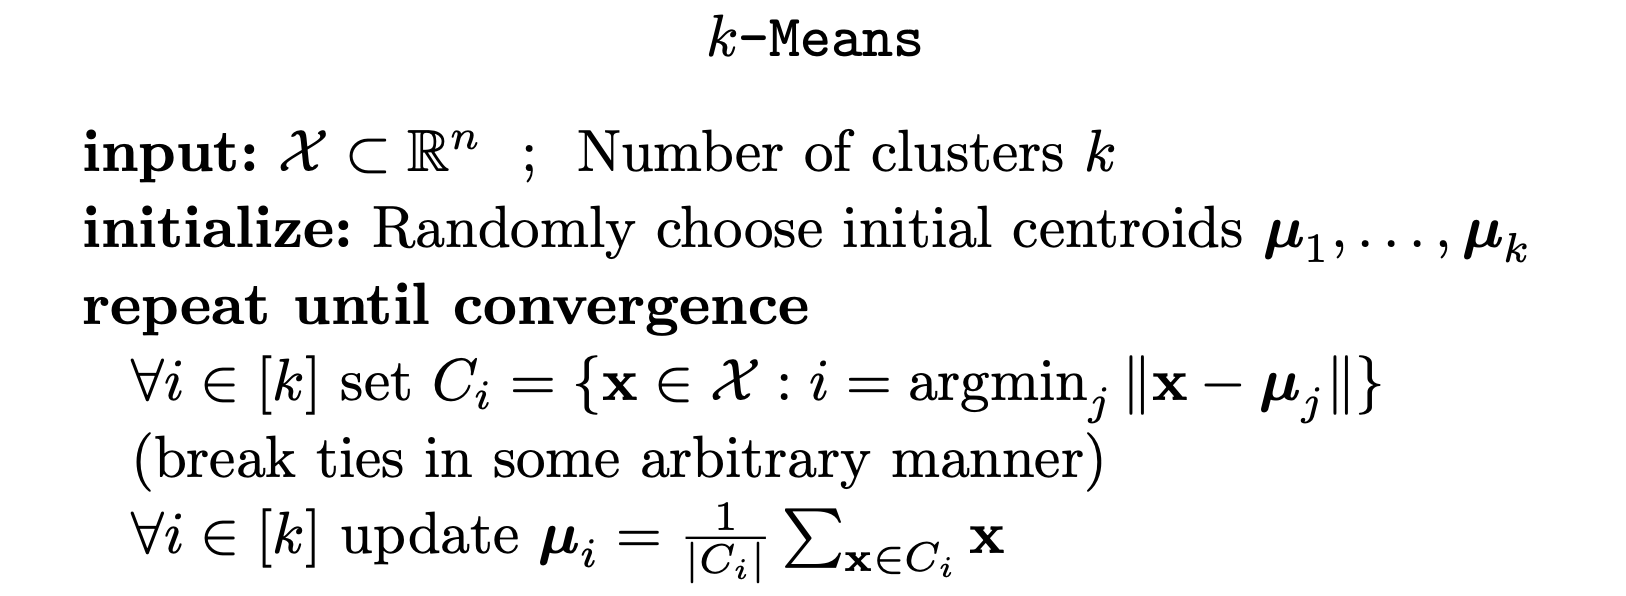
\includegraphics[width=0.65\textwidth]{assets/kmeans.png}
    \end{center}
    Example: 参考上课slides。
\end{frame}

\begin{frame}{K-means: Lloyd's method}
\begin{itemize}
    \item 重要性质:每一次迭代过程中,objective function 
    \[
        G_{\text{K-means}}((X, d), (C_1, C_2, \cdots, C_k)) =\min_{\mu_1, \mu_2, \cdots, \mu_k} \sum_{i=1}^{k} \sum_{x \in C_i} d(x, \mu_i) ^{2}
    \]
    不会增加。
    \item Note: Lloyd's method是最常用的一种K-means算法,但K-means算法还有很多其他变种。
\end{itemize}
\end{frame}

\begin{frame}{Spectral Clustering}
    \begin{itemize}
        \item 思想:用 similarity graph $G$ 表示集合 $X = \left\{ x_1, x_2, \cdots, x_m \right\}$各点之间的关系。$G=(V, E)$,其中$V=\left\{ x_1, x_2, \cdots, x_m \right\} $, 每两个顶点之间连接一条权重为$W_{ij} = s(x_i, x_j)$的边,$s$是相似度度量,例如$s(x_i, x_j) = \exp\left( \frac{d(x_i, x_j)^{2}}{\sigma^{2}} \right) $
        \item Clustering问题可表述为:希望找到一种partition,同一part各点之间边权重较大,不同part各点之间边权重较小。
        \item 最小化 $Cut(C_1, C_2, \cdots, C_k) = \sum_{i=1}^{k} \sum_{r \in C_i, s \notin C_i} W_{rs}$ 经常会将单独一个点作为一个part。
        \item 解决办法:最小化 $RatioCut(C_1, C_2, \cdots, C_k) = \sum_{i=1}^{k} \frac{\sum_{r \in C_i, s \notin C_i} W_{rs}}{|C_i|}$,权衡part大小和part间边权重。
    \end{itemize}
\end{frame}

\begin{frame}{Spectral Clustering Analysis}
    \begin{block}{Definition: Unnormalized Graph Laplacian}
        一个有向图的unnormalized graph Laplacian定义为$L = D - W$,其中$D$是degree matrix,$D_{ii} = \sum_{j=1}^{m} W_{ij}$,$W$是边权重矩阵,对角元均为$0$。
    \end{block}
    \begin{block}{Lemma}
        设 $C = \left\{ C_1, C_2, \cdots, C_k \right\} $是一个clustering,定义$H \in \mathbb{R}^{m\times k}$:
        \[
            H_{ij} = \frac{1}{\sqrt{|C_j|}} \mathbbm 1[i \in C_j]
        \]
        则 $H^{T}H = I^{k\times k}$且$\text{RatioCut}(C_1, C_2, \cdots, C_k) = \text{tr}(H^{T}LH)$, 其中 $L$ 是similarity graph 的 unnormalized graph Laplacian.
    \end{block}
    证明思路:用$H$和$L$的定义直接得到。
\end{frame}

\begin{frame}{Spectral Clustering Analysis}
    根据上述Lemma,我们可以将RatioCut问题转化为如下问题:

    问题1 (original): 找一个矩阵$H \in \mathbb{R}^{m\times k}$,满足
    \begin{itemize}
        \item $H^{T}H = I$
        \item $H_{ij}=0$或$1/\sqrt{|C_j|}$
        \item 最小化 $\text{tr}(H^{T}LH)$
    \end{itemize}

    以上问题是一个integer programming problem,无法高效求解。所以对问题进行relax:

    问题2 (relax): 找一个矩阵$H \in \mathbb{R}^{m\times k}$,满足
    \begin{itemize}
        \item $H^{T}H = I$
        \item 最小化 $\text{tr}(H^{T}LH)$
    \end{itemize}
    这时问题变为标准的 PCA 问题,其解为$L$的对应前$k$个最小本征值的特征向量。
\end{frame}

\begin{frame}{Spectral Clustering Algorithm}
    算法:
    \begin{center}
        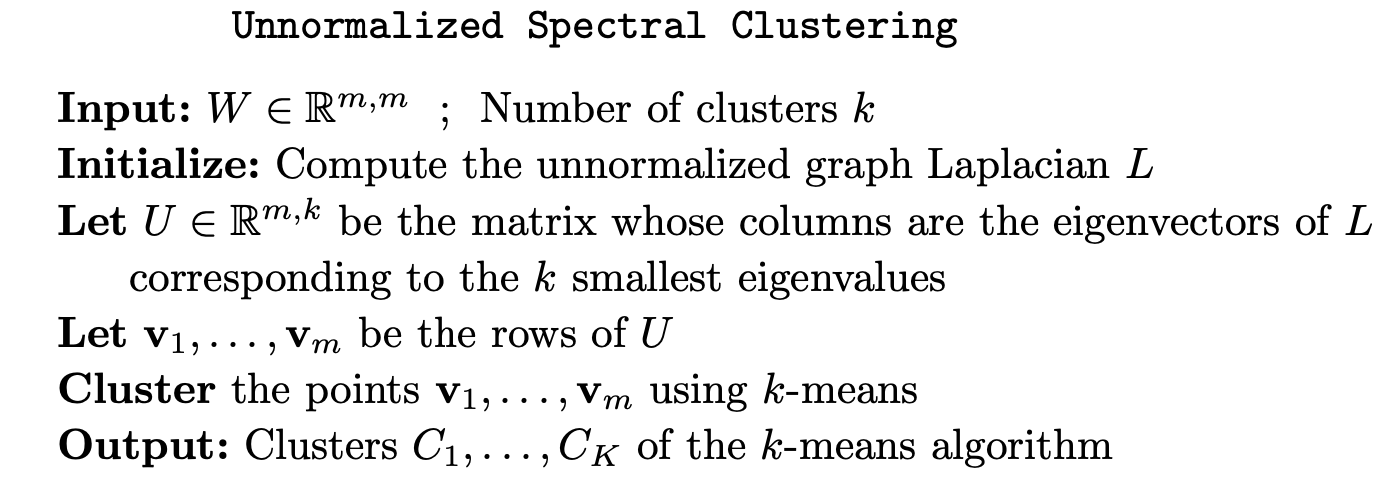
\includegraphics[width=0.7\textwidth]{assets/usc.png}
    \end{center}
\end{frame}

\begin{frame}{Birkhoff's Theorem}
    TODO
\end{frame}
